% Case study, caida data analysis
\subsubsection{CAIDA Telescope}
\label{sec:caida}

The UC San Diego network telescope maintained by CAIDA consists of a globally
routed /8 network that carries almost no legitimate traffic. After filtering
out the legitimate traffic, the resulting data provides a snapshot of anomalous
traffic to about 1/256th of all IPv4 addresses on the Internet. This traffic,
called Internet Background Radiation (IBR)~\cite{pang2004characteristics},
has been used by researchers to study worms, DDoS attacks~\cite{moore2006inferring}
and Internet scanning. Benson~\etal~\cite{benson2015leveraging} have collected
scanning traffic from the telescope from 2014 to July 2016 using the default
parameters of the Bro IDS~\cite{BroNetwork} to identify scanning traffic, namely,
the same source IP address is used to contact 25 unique destination IP addresses
on the same destination port/protocol within 5 minutes.

We use the scanners detected by the UC San Diego network telescope as a large
scan feed, and compare its data with the threat intelligence scan
feeds. Since the telescope is listening on a very large IP address
range (over 16 million addresses), if there is an indiscriminate
scanner observed by threat intel feeds, then this scanner will likely
also be observed by the telescope.

%Therefore, we use telescope's data as the grand truth and try to measure the quality of our scan feeds' data.

We use the scanners detected by the telescope from January 2016 to
July 2016, which consists of 27,047,066 IP addresses. The total amount
of IPs in all the scan threat intelligence feeds during this period is
675,243, which covers only 0.6\%(175,496 shared IPs) of all the
telescope scan IPs. This is not a surprise, considering the large volume
difference. On the other hand, however, telescope scanners only share 25.9\%
of all the feeds' data, which means majority of IPs in scan feeds are not
captured by the telescope. Table~\ref{tab:caida_ip_overlap} shows
the intersection of each feed and the telescope. For the two largest
feeds, {\feedTSSnort} and {\feedetiprep}, the intersections are
relatively low: 18\% and 22\%, respectively.
For the small feeds, their intersection rates are
comparably higher, but there is still a non-trivial proportion of a feed
that does not appear in the telescope.

%with exceptions like {\feedTSAnalyst} and {\feedFBZendesk}. %This result
%contradicts with our expectation, as we were expecting more intersection
%on the big scan feeds like {\feedetiprep}.

\begin{table}
\small
\caption{Intersection between scan feeds and telescope scanners.
\textit{Volume} contains the total amount of IPs in each feed from
Jan. 2016 to July 2016. \textit{Intersection} is the proportion
of each feed's IPs that overlap with the telescope data.}
\centering
 \resizebox{0.7\linewidth}{!}{
\begin{tabular}{l r r }
\toprule
Feed & Volume & Intersection \\
\midrule
{PA Snort BlockList}     & 312,533   & 18.2\% \\
%{\feedetiprep}           & 293,484   & 22.1\% \\
%{\feedpacketmail}        & 50,723    & 83.6\% \\
%{PA Packetmail ramnode}  & 11,452    & 76.1\% \\
%{\feedalienvault}        & 8,695     & 35.1\% \\
%{PA Malicious IPs}       & 7,960     & 63.3\% \\
%{PA Packetmail CARISIT}  & 5,955     & 71.5\%\\
%{PA SANS Top IPs}        & 3,087     & 77.4\%\\
%{PA Analyst}             & 444       & 52.0\%\\
%{PA Shockpot IPs}        & 156       & 50.0\%\\
%{PA SANS IPs}            & 129       & 63.6\%\\
%{FB Aggregator}          & 103       & 37.9\%\\
\midrule
%Total & 675,243 & 25.9\%\\
\bottomrule
\end{tabular}
}
\label{tab:caida_ip_overlap}
\end{table}

To further understand how well each scan feed detects scanning
activities, we measure how different sizes of scanners in the
telescope are covered by each feed. Here, \emph{scanner size} means how
many IPs a scanner has scanned in the telescope within a
day. Figure~\ref{fig:caida_coverage_cdf} shows the coverage rate of
each feed over different sizes of scanners, ranging from 1,000 to 10
million. (There are 7,038,999 IPs whose sizes are over 1,000, 38,170
IPs are over 100,000 and 3,713 IPs are over 10 million.) The graph
shows that, as the scanner size increases, the coverage of most feeds
over the datasets also increases. When comparing across feeds, the
large feeds tend to cover a substantial amount of big scanners but
small feeds' coverage is very limited. Feed {\feedpacketmail}, for
example, covers close to 40\% of all the scanners that have scanned
over 1 million IPs in the telescope, and it has better coverage than
{\feedetiprep}, whose volume is much larger. Feed {\feedTSSnort},
however, has a surprisingly low intersection with big scanners
comparing with its large volume. Considering its low intersection with
other scan feeds, we suspect that most data in this feed is not real
Internet scanners.

There are two bumps in multiple lines in
Figure~\ref{fig:caida_coverage_cdf} around the 100K mark. By inspecting
the data we found that the volume of scanners in telescope quickly
reduces 45\% after the scan size threshold increases from 64K to 66K,
and reduces 21\% again after the threshold increases from 129K to 132K.
The overlapped amount with feeds do not change very much in the process,
which results in two bumps on the coverage rate. These two ranges very
closely encapsulate $2^{16}$ and $2^{17}$. We suspect this is related to
the underlying patterns of scanning activities.


\begin{figure}
\centering
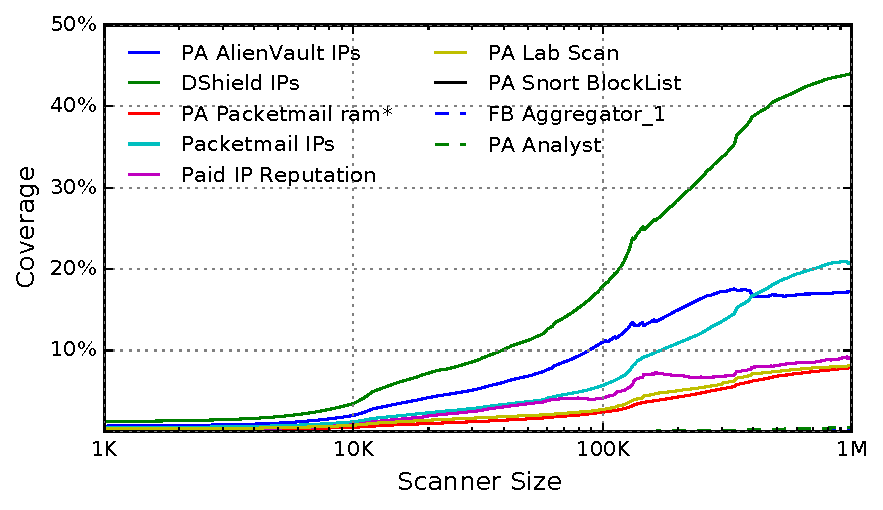
\includegraphics[width=\linewidth]{images/caida_coverage_cdf.pdf}
\caption{The coverage of each feed on different sizes of scanners,
showing the proportion of scanners of a given size (or larger) are
covered by each feed.}
\label{fig:caida_coverage_cdf}
\end{figure}

\finding\ The union of all the scan IPs in the feeds covers less than
1\% of the scanners collected by the telescope. Even if we only look
at the scanners with sizes larger than 1,000, the coverage is still
below 1\%. This result suggests the coverage capability of scan feeds
is very limited. Using another metric, the volume of scanners in the
telescope is over 20 times larger than that of the scan feeds, yet the
telescope scanners only cover 25.9\% of all of the scanning feeds'
data. The overall volume of scanning activities is so extensive that
even a /8 telescope will miss many of them, particularly if scanners
are selective in targets (avoiding or focusing on certain IP ranges)
or rate limits (falling below scanner labeling thresholds). The
coverage curve based on scanner sizes showed that scan feeds are
better at capturing large scanners, which is intuitive, but that a
larger feed does not necessarily mean better coverage.


%\begin{figure}
%\centering
%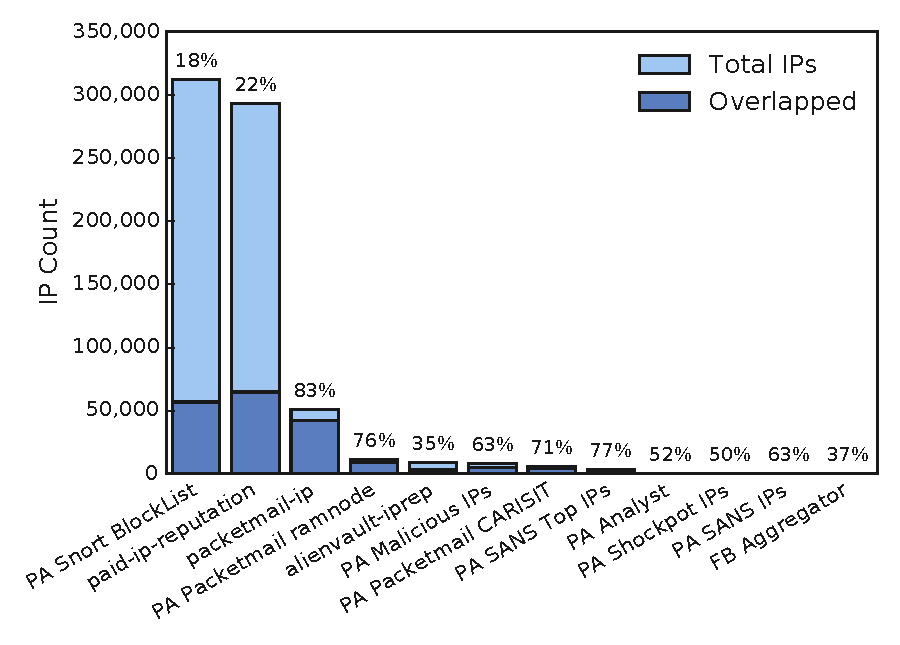
\includegraphics[width=0.95\linewidth]{images/caida_ip_overlap.pdf}
%\caption{Overall intersection between telescope scanners IPs and scan feeds IPs. The numbers on top of each bar are the intersection rate.}
%\label{fig:caida_ip_overlap}
%\end{figure}

%Figure~\ref{fig:caida_daily_overlap} shows the daily intersection between telescope scan data and every scan feed, and the number is calculated using a 7-day sliding window. The graph shows that the intersection between 6 feeds and telescope data are fairly stable over the time: the daily intersection rates of feed {\feedpacketmail}, {\feedTSramnode}, {\feedTScarisit} and {\feedTSSANS} stay roughly around 60\%, and feed {\feedetiprep} and {\feedalienvault}'s intersection rates stay around 20\%. There are 5 scan feeds we didn't show in this graph since their intersection rates fluctuate radically over the time.

%\begin{figure}
%\centering
%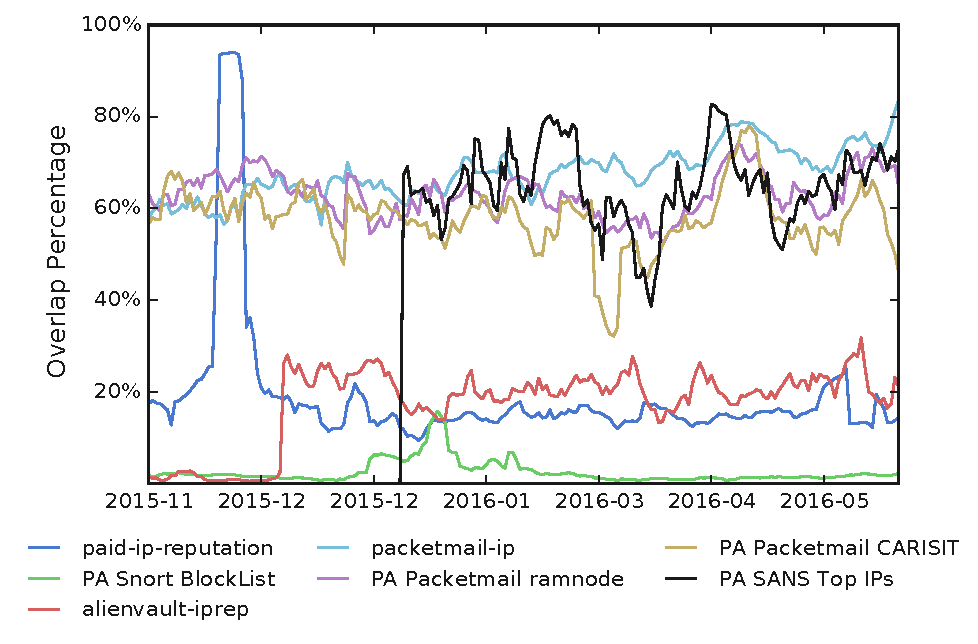
\includegraphics[width=0.95\linewidth]{images/caida_daily_overlap.pdf}
%\caption{Daily intersection between telescope scanners IPs and scan feeds. The percentage represents how much of each feed's data is overlapped with telescope's data on the same days}
%\label{fig:caida_daily_overlap}
%\end{figure}


%Internet scanning is usually captured through listening on certain IP ranges that are not supposed to receive legitimate traffic like Internet telescope does. Big scan feeds are probably the ones that listen on large IP ranges while small feeds are listening on small ranges. If an Internet scanning is captured by a small scan feed, then the scanner is probably conducting a large scale Internet scan, which will also likely hit one of the UCSD network telescope's IP addresses. That's why small feeds have relatively high intersection with telescope data. Likewise, big scan feeds tend to capture more small scanners that not always hit the telescope, resulting in low intersection rates. The stable over the time intersection rates in Figure~\ref{fig:caida_daily_overlap} further proofs that these feeds collect their data in the same fashion as the telescope does. The feeds whose daily intersection rate fluctuate all the times means their data are probably not collected in this passive listening fashion.

\iffalse
\begin{table}
\small
\caption{Scan feeds' coverage of large scanners}
\centering
 \resizebox{\linewidth}{!}{
\begin{tabular}{l l l l l l}
\toprule
Feed & 100K & 250K & 500K & 1M & 2M\\
\midrule
{\feedetiprep}             & 19.75\%     & 40.38\%   & 38.61\% & 38.44\%  & 41.44\%\\
{\feedpacketmail}          & 8.28\%      & 24.46\%   & 31.33\% & 36.53\%  & 38.84\%\\
{\feedTScarisit}           & 2.59\%      & 9.19\%    & 11.99\% & 14.66\%  & 16.46\%\\
{\feedTSramnode}           & 2.39\%      & 7.59\%    & 9.66\%  & 11.60\%  & 12.68\%\\
{\feedTSMalicious}         & 2.73\%      & 7.26\%    & 9.51\%  & 10.42\%  & 9.89\%\\
{\feedTSSANS}              & 3.05\%      & 7.06\%    & 8.79\%  & 10.30\%  & 11.22\%\\
{\feedalienvault}          & 2.52\%      & 7.96\%    & 9.76\%  & 11.50\%  & 13.06\%\\
{\feedTSSnort}             & 0.34\%      & 0.61\%    & 0.74\%  & 0.72\%   & 0.48\%\\
{PA SANS IPs}              & 0.13\%      & 0.53\%    & 0.71\%  & 0.92\%   & 1.06\%\\
{\feedTSAnalyst}           & 0.10\%      & 0.41\%    & 0.56\%  & 0.64\%   & 0.62\%\\
{\feedTSShockpot}          & 0.05\%      & 0.14\%    & 0.11\%  & 0.10\%   & 0.10\%\\
{\feedFBZendesk}           & 0.04\%      & 0.18\%    & 0.24\%  & 0.30\%   & 0.40\%\\
\midrule
Dataset Size & 91,624 & 20,827 & 14,908 & 11,196 & 9,007 \\
\bottomrule
\end{tabular}
}
\label{tab:bulk_scan_overlap}
\end{table}
\fi
